\documentclass{article}


\usepackage{amsmath}
\usepackage{amsfonts}
\usepackage{stmaryrd}
\usepackage{geometry}
\usepackage{graphicx}
\usepackage{float}
\usepackage{appendix}
\usepackage{pdfpages}

\geometry{hmargin = 2.5cm, vmargin = 1.5cm}

\title{IEOR 241 : Homework 9}
\author{Arnaud Minondo}
\begin{document}
\maketitle
For each of the exercises you can find the code in the corresponding appendix.
\section*{Exercise 1}
\textbf{1.} What I obtained from simulating a uniform on $[0;1]$ 5 times is : 0.56, 0.8, 0.78, 0.8, 0.1
\\\\
\textbf{2.} What I obtained as a mean estimate is 0.51.
\section*{Exercise 2}
\textbf{1.} Let $U \sim \mathcal{U}([0;1])$ and define $V = 2\pi U$.
\\
$\forall t \in [0;2\pi]$, $\mathbb{P}(V\leq t) = \mathbb{P}(U\leq \frac{t}{2\pi}) = \frac{t}{2\pi}$.
\\
Hence $$\boxed{f_V(v) = \left\{\begin{array}{ll}
    0 & \text{if } t\in]-\infty;0]\cup[2\pi;\infty[\\
    \frac{1}{2\pi} & \text{otherwise}
\end{array}\right. \text{ and } V\sim\mathcal{U}([0;2\pi])}$$
\\\\
\textbf{2.} $$\boxed{\text{The mean estimate for $V$ is 3.15 which is very close to $\pi$}}$$.
\section*{Exercise 3}
\textbf{1.} The exponential distribution $\mathcal{E}(\frac{1}{2})$ has the distribution function $F(t) = 1-e^{-\frac{1}{2}t}$ with $F^{-1}(x) = -2\ln(1-x)$.
Let $E = F^{-1}(U)$ then $\mathbb{P}(E\leq t) = \mathbb{P}(U\leq F(t)) = F(t)$ and $E\sim \mathcal{E}(\frac{1}{2})$. $$\boxed{\text{Sampling 5 times I obtained : 0.55, 3.03, 1.91, 0.36, 0.55}}$$
\textbf{2.} $$\boxed{\text{The estimated mean value of $E$ is : 2.02 which is very close to 2} }$$
\newpage
\section*{Exercise 4}
\textbf{1.} We can see in figure 1 that $N_1 = \sqrt{E}\cos(V)$ follows a gaussian distribution.
\begin{figure}[H]
    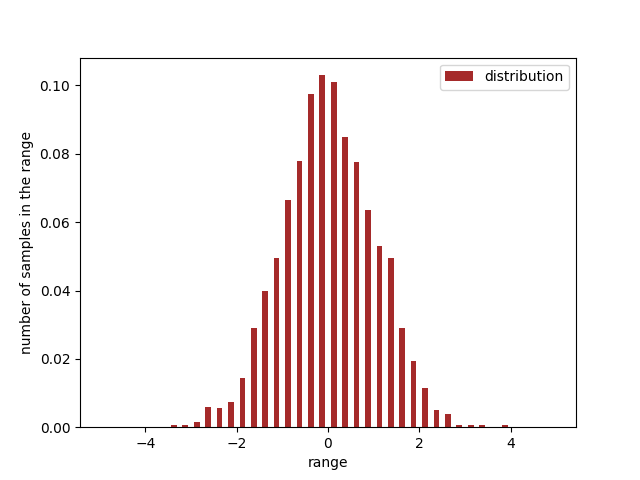
\includegraphics[width = 9cm, height = 7cm]{img/uniform_to_gaussian.png}
    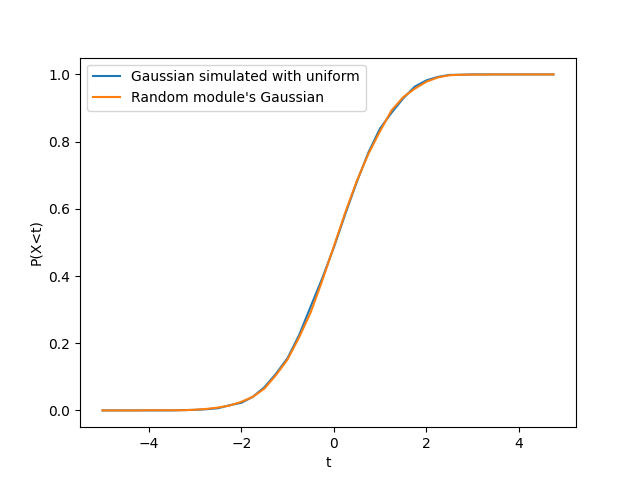
\includegraphics[width = 9cm, height = 7cm]{img/comparison.png}
    \caption{On the left : Density of the simulated gaussian. On the right comparison of the distribution function between the random python's module gaussian and our uniform simulated gaussia.n}
\end{figure}
\noindent A few samples from $N_1$ are : [-0.05, 0.45, -0.04, 0.32, 0.6] and for $N_2$ : [0.47, -0.43, 1.77, -0.28, -1.08]
\\\\
\textbf{2.} $$\boxed{\text{The two means etimate are 0.2 which is very close to 0}}$$
\section*{Exercise 5}
\textbf{1.} We need $X = \mu_X + \sigma_XN_1$ and $Y = \mu_Y+ \rho \sigma_YN_1+ \sigma_Y \sqrt{1-\rho^2}N_2$
 ie. $$\boxed{X= 1+N_1\text{ and }Y = 1.5+ N_1+ 2\sqrt{0.75}N_2}$$
\\\\
\textbf{2.} The estimated mean for X is : 1.01 and for Y is : 1.56 both are very close to there respective mean. The estimated correlation is 0.54 which is very close to $\rho$.
\begin{figure}[H]
    \begin{center}
        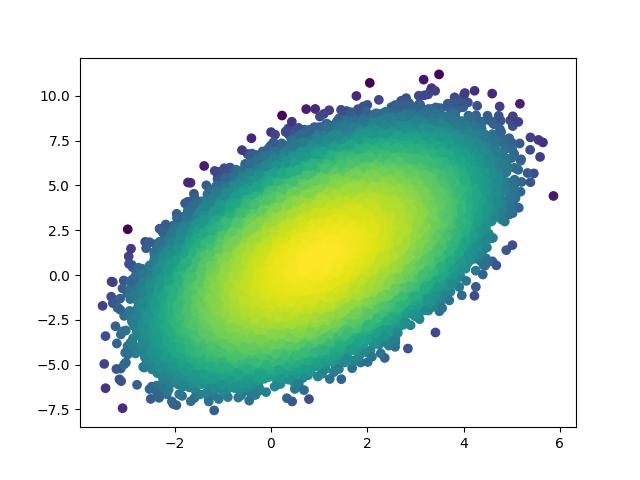
\includegraphics[width = 9cm]{img/Gaussian_Cholevsky.png}
    \end{center}
    \label{label:Gaussian_cholevsky}
    \caption{Simulated distribution of correlated gaussians $X$ and $Y$}
\end{figure}
\begin{appendix}
    \section{notebook.ipynb}
    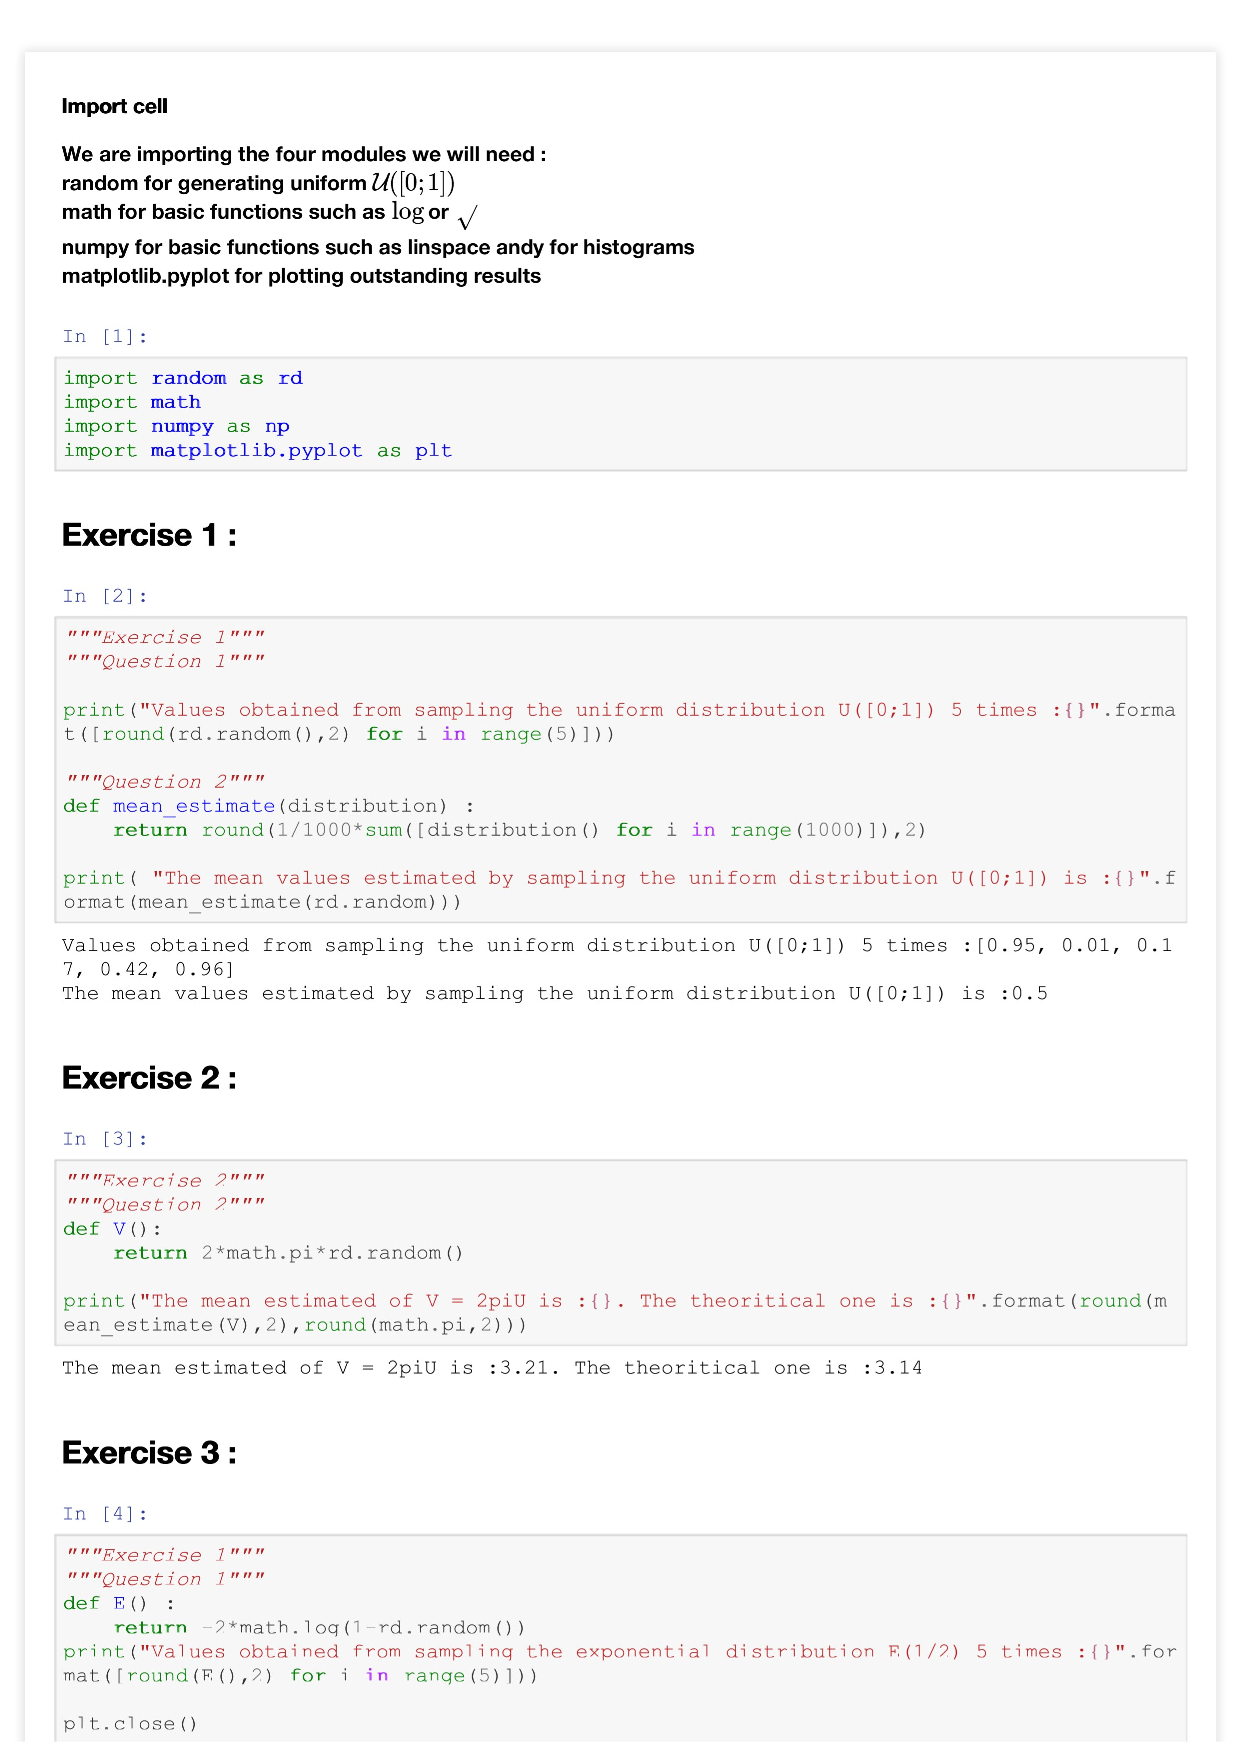
\includepdf[pages=-]{img/notebook.pdf}
\end{appendix}
\end{document}